% Created by tikzDevice version 0.12.6 on 2024-03-15 15:16:37
% !TEX encoding = UTF-8 Unicode
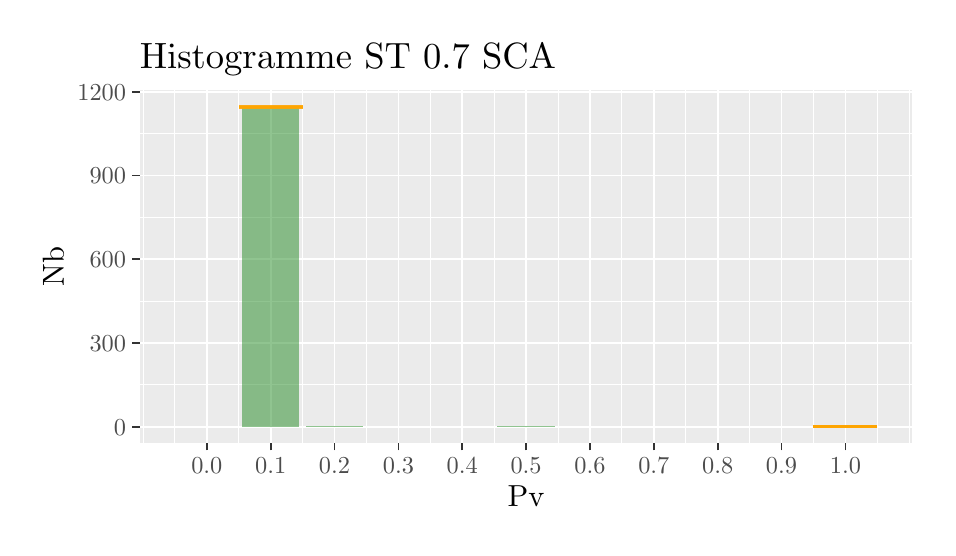
\begin{tikzpicture}[x=1pt,y=1pt]
\definecolor{fillColor}{RGB}{255,255,255}
\path[use as bounding box,fill=fillColor,fill opacity=0.00] (0,0) rectangle (325.21,180.67);
\begin{scope}
\path[clip] (  0.00,  0.00) rectangle (325.21,180.67);
\definecolor{drawColor}{RGB}{255,255,255}
\definecolor{fillColor}{RGB}{255,255,255}

\path[draw=drawColor,line width= 0.6pt,line join=round,line cap=round,fill=fillColor] (  0.00,  0.00) rectangle (325.21,180.68);
\end{scope}
\begin{scope}
\path[clip] ( 40.51, 30.69) rectangle (319.71,158.02);
\definecolor{fillColor}{gray}{0.92}

\path[fill=fillColor] ( 40.51, 30.69) rectangle (319.71,158.02);
\definecolor{drawColor}{RGB}{255,255,255}

\path[draw=drawColor,line width= 0.3pt,line join=round] ( 40.51, 51.60) --
	(319.71, 51.60);

\path[draw=drawColor,line width= 0.3pt,line join=round] ( 40.51, 81.86) --
	(319.71, 81.86);

\path[draw=drawColor,line width= 0.3pt,line join=round] ( 40.51,112.12) --
	(319.71,112.12);

\path[draw=drawColor,line width= 0.3pt,line join=round] ( 40.51,142.38) --
	(319.71,142.38);

\path[draw=drawColor,line width= 0.3pt,line join=round] ( 41.66, 30.69) --
	( 41.66,158.02);

\path[draw=drawColor,line width= 0.3pt,line join=round] ( 53.20, 30.69) --
	( 53.20,158.02);

\path[draw=drawColor,line width= 0.3pt,line join=round] ( 76.28, 30.69) --
	( 76.28,158.02);

\path[draw=drawColor,line width= 0.3pt,line join=round] ( 99.35, 30.69) --
	( 99.35,158.02);

\path[draw=drawColor,line width= 0.3pt,line join=round] (122.43, 30.69) --
	(122.43,158.02);

\path[draw=drawColor,line width= 0.3pt,line join=round] (145.50, 30.69) --
	(145.50,158.02);

\path[draw=drawColor,line width= 0.3pt,line join=round] (168.58, 30.69) --
	(168.58,158.02);

\path[draw=drawColor,line width= 0.3pt,line join=round] (191.65, 30.69) --
	(191.65,158.02);

\path[draw=drawColor,line width= 0.3pt,line join=round] (214.72, 30.69) --
	(214.72,158.02);

\path[draw=drawColor,line width= 0.3pt,line join=round] (237.80, 30.69) --
	(237.80,158.02);

\path[draw=drawColor,line width= 0.3pt,line join=round] (260.87, 30.69) --
	(260.87,158.02);

\path[draw=drawColor,line width= 0.3pt,line join=round] (283.95, 30.69) --
	(283.95,158.02);

\path[draw=drawColor,line width= 0.3pt,line join=round] (307.02, 30.69) --
	(307.02,158.02);

\path[draw=drawColor,line width= 0.3pt,line join=round] (318.56, 30.69) --
	(318.56,158.02);

\path[draw=drawColor,line width= 0.6pt,line join=round] ( 40.51, 36.47) --
	(319.71, 36.47);

\path[draw=drawColor,line width= 0.6pt,line join=round] ( 40.51, 66.73) --
	(319.71, 66.73);

\path[draw=drawColor,line width= 0.6pt,line join=round] ( 40.51, 96.99) --
	(319.71, 96.99);

\path[draw=drawColor,line width= 0.6pt,line join=round] ( 40.51,127.25) --
	(319.71,127.25);

\path[draw=drawColor,line width= 0.6pt,line join=round] ( 40.51,157.51) --
	(319.71,157.51);

\path[draw=drawColor,line width= 0.6pt,line join=round] ( 64.74, 30.69) --
	( 64.74,158.02);

\path[draw=drawColor,line width= 0.6pt,line join=round] ( 87.81, 30.69) --
	( 87.81,158.02);

\path[draw=drawColor,line width= 0.6pt,line join=round] (110.89, 30.69) --
	(110.89,158.02);

\path[draw=drawColor,line width= 0.6pt,line join=round] (133.96, 30.69) --
	(133.96,158.02);

\path[draw=drawColor,line width= 0.6pt,line join=round] (157.04, 30.69) --
	(157.04,158.02);

\path[draw=drawColor,line width= 0.6pt,line join=round] (180.11, 30.69) --
	(180.11,158.02);

\path[draw=drawColor,line width= 0.6pt,line join=round] (203.19, 30.69) --
	(203.19,158.02);

\path[draw=drawColor,line width= 0.6pt,line join=round] (226.26, 30.69) --
	(226.26,158.02);

\path[draw=drawColor,line width= 0.6pt,line join=round] (249.34, 30.69) --
	(249.34,158.02);

\path[draw=drawColor,line width= 0.6pt,line join=round] (272.41, 30.69) --
	(272.41,158.02);

\path[draw=drawColor,line width= 0.6pt,line join=round] (295.49, 30.69) --
	(295.49,158.02);
\definecolor{fillColor}{RGB}{34,139,34}

\path[fill=fillColor,fill opacity=0.50] ( 77.43, 36.47) rectangle ( 98.20,152.02);

\path[fill=fillColor,fill opacity=0.50] (100.50, 36.47) rectangle (121.27, 36.83);

\path[fill=fillColor,fill opacity=0.50] (169.73, 36.47) rectangle (190.50, 36.68);

\path[fill=fillColor,fill opacity=0.50] (285.10, 36.47) rectangle (305.87, 36.57);
\definecolor{drawColor}{RGB}{255,165,0}

\path[draw=drawColor,draw opacity=0.90,line width= 0.9pt,line join=round] ( 76.28,152.23) --
	( 99.35,152.23);

\path[draw=drawColor,draw opacity=0.90,line width= 0.9pt,line join=round] ( 87.81,152.23) --
	( 87.81,151.80);

\path[draw=drawColor,draw opacity=0.90,line width= 0.9pt,line join=round] ( 76.28,151.80) --
	( 99.35,151.80);

\path[draw=drawColor,draw opacity=0.90,line width= 0.9pt,line join=round] (283.95, 36.57) --
	(307.02, 36.57);

\path[draw=drawColor,draw opacity=0.90,line width= 0.9pt,line join=round] (295.49, 36.57) --
	(295.49, 36.57);

\path[draw=drawColor,draw opacity=0.90,line width= 0.9pt,line join=round] (283.95, 36.57) --
	(307.02, 36.57);
\end{scope}
\begin{scope}
\path[clip] (  0.00,  0.00) rectangle (325.21,180.67);
\definecolor{drawColor}{gray}{0.30}

\node[text=drawColor,anchor=base east,inner sep=0pt, outer sep=0pt, scale=  0.88] at ( 35.56, 33.44) {0};

\node[text=drawColor,anchor=base east,inner sep=0pt, outer sep=0pt, scale=  0.88] at ( 35.56, 63.70) {300};

\node[text=drawColor,anchor=base east,inner sep=0pt, outer sep=0pt, scale=  0.88] at ( 35.56, 93.96) {600};

\node[text=drawColor,anchor=base east,inner sep=0pt, outer sep=0pt, scale=  0.88] at ( 35.56,124.22) {900};

\node[text=drawColor,anchor=base east,inner sep=0pt, outer sep=0pt, scale=  0.88] at ( 35.56,154.48) {1200};
\end{scope}
\begin{scope}
\path[clip] (  0.00,  0.00) rectangle (325.21,180.67);
\definecolor{drawColor}{gray}{0.20}

\path[draw=drawColor,line width= 0.6pt,line join=round] ( 37.76, 36.47) --
	( 40.51, 36.47);

\path[draw=drawColor,line width= 0.6pt,line join=round] ( 37.76, 66.73) --
	( 40.51, 66.73);

\path[draw=drawColor,line width= 0.6pt,line join=round] ( 37.76, 96.99) --
	( 40.51, 96.99);

\path[draw=drawColor,line width= 0.6pt,line join=round] ( 37.76,127.25) --
	( 40.51,127.25);

\path[draw=drawColor,line width= 0.6pt,line join=round] ( 37.76,157.51) --
	( 40.51,157.51);
\end{scope}
\begin{scope}
\path[clip] (  0.00,  0.00) rectangle (325.21,180.67);
\definecolor{drawColor}{gray}{0.20}

\path[draw=drawColor,line width= 0.6pt,line join=round] ( 64.74, 27.94) --
	( 64.74, 30.69);

\path[draw=drawColor,line width= 0.6pt,line join=round] ( 87.81, 27.94) --
	( 87.81, 30.69);

\path[draw=drawColor,line width= 0.6pt,line join=round] (110.89, 27.94) --
	(110.89, 30.69);

\path[draw=drawColor,line width= 0.6pt,line join=round] (133.96, 27.94) --
	(133.96, 30.69);

\path[draw=drawColor,line width= 0.6pt,line join=round] (157.04, 27.94) --
	(157.04, 30.69);

\path[draw=drawColor,line width= 0.6pt,line join=round] (180.11, 27.94) --
	(180.11, 30.69);

\path[draw=drawColor,line width= 0.6pt,line join=round] (203.19, 27.94) --
	(203.19, 30.69);

\path[draw=drawColor,line width= 0.6pt,line join=round] (226.26, 27.94) --
	(226.26, 30.69);

\path[draw=drawColor,line width= 0.6pt,line join=round] (249.34, 27.94) --
	(249.34, 30.69);

\path[draw=drawColor,line width= 0.6pt,line join=round] (272.41, 27.94) --
	(272.41, 30.69);

\path[draw=drawColor,line width= 0.6pt,line join=round] (295.49, 27.94) --
	(295.49, 30.69);
\end{scope}
\begin{scope}
\path[clip] (  0.00,  0.00) rectangle (325.21,180.67);
\definecolor{drawColor}{gray}{0.30}

\node[text=drawColor,anchor=base,inner sep=0pt, outer sep=0pt, scale=  0.88] at ( 64.74, 19.68) {0.0};

\node[text=drawColor,anchor=base,inner sep=0pt, outer sep=0pt, scale=  0.88] at ( 87.81, 19.68) {0.1};

\node[text=drawColor,anchor=base,inner sep=0pt, outer sep=0pt, scale=  0.88] at (110.89, 19.68) {0.2};

\node[text=drawColor,anchor=base,inner sep=0pt, outer sep=0pt, scale=  0.88] at (133.96, 19.68) {0.3};

\node[text=drawColor,anchor=base,inner sep=0pt, outer sep=0pt, scale=  0.88] at (157.04, 19.68) {0.4};

\node[text=drawColor,anchor=base,inner sep=0pt, outer sep=0pt, scale=  0.88] at (180.11, 19.68) {0.5};

\node[text=drawColor,anchor=base,inner sep=0pt, outer sep=0pt, scale=  0.88] at (203.19, 19.68) {0.6};

\node[text=drawColor,anchor=base,inner sep=0pt, outer sep=0pt, scale=  0.88] at (226.26, 19.68) {0.7};

\node[text=drawColor,anchor=base,inner sep=0pt, outer sep=0pt, scale=  0.88] at (249.34, 19.68) {0.8};

\node[text=drawColor,anchor=base,inner sep=0pt, outer sep=0pt, scale=  0.88] at (272.41, 19.68) {0.9};

\node[text=drawColor,anchor=base,inner sep=0pt, outer sep=0pt, scale=  0.88] at (295.49, 19.68) {1.0};
\end{scope}
\begin{scope}
\path[clip] (  0.00,  0.00) rectangle (325.21,180.67);
\definecolor{drawColor}{RGB}{0,0,0}

\node[text=drawColor,anchor=base,inner sep=0pt, outer sep=0pt, scale=  1.10] at (180.11,  7.64) {Pv};
\end{scope}
\begin{scope}
\path[clip] (  0.00,  0.00) rectangle (325.21,180.67);
\definecolor{drawColor}{RGB}{0,0,0}

\node[text=drawColor,rotate= 90.00,anchor=base,inner sep=0pt, outer sep=0pt, scale=  1.10] at ( 13.08, 94.35) {Nb};
\end{scope}
\begin{scope}
\path[clip] (  0.00,  0.00) rectangle (325.21,180.67);
\definecolor{drawColor}{RGB}{0,0,0}

\node[text=drawColor,anchor=base west,inner sep=0pt, outer sep=0pt, scale=  1.32] at ( 40.51,166.08) {Histogramme ST 0.7 SCA};
\end{scope}
\end{tikzpicture}
